\section{Introduction}
The growth of CdTe on oxide substrates, specifically single crystal sapphire, has been a 
region of great interest for the Preston research group. Work has been published on 
optimization of growth parameters, the role of lattice constants, and the optical 
properties of the resulting thin films\cite{Neretina2009a,Neretina2008b,Neretina2009b,Neretina2007,Neretina2006,cdte-optical}.

While the work investigating the growth parameters and properties of the resulting thin 
films has progressed to a high level, relatively less investigation has been focused on 
explaining the surprising success that has been achieved with this material system. With 
a relative lattice mismatch of 3.xx\% between CdTe and sapphire, a difference in the 
crystallographic space group (cubic CdTe versus hexagonal sapphire), and a vast chemical 
difference (high ionicity semiconductor CdTe versus complex oxide sapphire), the high 
quality single crystal nature of the grown thin films is far from expected.

In this work investigating the CdTe on sapphire heteroepitaxial material system, the 
unexpected high quality growth is examined through the lens of symmetry and energy at the 
epitaxial 
interface. These examinations reveal theoretical support for an explanatory model of the 
epitaxial alignment 
and defects present in CdTe thin films. These examinations also reveal the previously 
undocumented and highly surprising result that CdTe is not bonded nearly as strongly as 
expected to the sapphire substrates after epitaxial growth, resulting in the 
technologically relevant liftoff phenomenon. The liftoff phenomon is examined and its 
resulting freestanding thin films are characterized. This liftoff phenomon has been 
discovered to be significantly robust as to apply for a provisional patent\cite{patent}. 
This work was completed in collaboration 
with Mr. Stephen M. Jovanovic (growths), Dr. Kristoffer Mienander (DFT, surfaces) and Ms. 
Steffi Woo (TEM), and relies on prior work by Dr. Robert Hughes and Dr. Svetlana Neretina.

\section{Background}\todo{Fill in numbers here}
CdTe is a cubic semiconductor (a = 6.14xxx) with a very strong propensity to grown 
(111)-up, that is 
alternating layers of cadnimum and telurium, regardless of the structure of the 
underlying substrate. Thus the key requirement for the growth of quality single crystal 
thin films is to control the nucleation and in-plane orientation. \textalpha-Al$_2$O$_3$ 
(sapphire) 
is a rhobehedral complex oxide (a = xxxx, c = yyy), which presents a hexgonal surface net 
on its c-plane surface. As had been previously investigated by the Preston research 
group, the (110) diagonal of CdTe matches to a lattice constant of sapphire to within 
3.xx\%, providing a geometric template for the epitaxial alignment of (111)-up on the 
c-plane surface. While the c-plane sapphire offers an epitaxial template for the CdTe, 
the mismatch of cubic on hexagonal symmetries offers two equivalent orientations for the 
CdTe crystal, as shown in \cref{fig:cdteliftoff_geometry}.
\begin{figure}
    \centering
    \missingfigure{Triangle on Hexagon Fit}
    \caption{\label{fig:cdteliftoff_geometry}Geometric model of cubic CdTe crystal 
    structure fit on hexagonal c-plane sapphire surface}
\end{figure}
Despite the geometric equivalence of two orientations of cubic on hexagonal symmetry, 
growths done by this research group have resulted in a single orientation of CdTe on the 
sapphire surface. Previous work by this research group attempted to explain the preferred 
orientation through experiments in the modification of sapphire\cite{Neretina2009b}, 
suggesting that the energy considerations at the surface play a key factor in epitaxy.
\section{Experimental}
CdTe thin films were deposited on single crystal c-plane \textalpha-Al$_2$O$_3$ $\pm$ 
0.5\degree wafers, obtained from MTI Crystals Inc and diced into 12 mm $\times$ 12 mm 
squares. Prior to deposition, substrates were solvent cleaned in an ultrasonic bath. 
Samples were loaded into a custom pulsed laser deposition chamber at a base pressure of 
1x10E-7 Torr and in-situ annealed at 450\degree\celsius for 30 minutes. CdTe thin films 
were deposited by pulsed laser deposition using a GSI Lumonics IPEX-848 KrF excimer laser 
with a wavelength of 248 nm. Pulses from the laser were focused and rastered radially 
onto a rotating CdTe 2.54 cm diameter target with a spot size of 4.25 
mm\textsuperscript{2} and average 
energy density of 1.8 J/cm\textsuperscript{2}. The CdTe 5N (99.999\%) pressed powder 
target obtained from 
Princeton Scientific was stoichiometric and undoped. During growth samples were kept at a 
nominal temperature of 300\degree\celsius via a Pt-Rh thermocouple on the growth furnace 
surface. 
Films were grown to a thickness of 100 nm, as determined by optical and stylus 
profilometry.

Structural information was obtained using 2DXRD techniques. A Bruker SMART6000 CCD 
detector on a Bruker 3-circle D8 goniometer with Rigaku RU-200 rotating anode X-ray 
generator and parallel-focusing mirror optics were used for the data collection. 2DXRD 
data was processed into pole figures using Bruker GADDS.
\section{Results and Discussion}
CdTe thin films had been previously thoroughly structurally characterized via 2DXRD, AFM 
and TEM. As such, one of the next steps to fully characterize the CdTe thin films was to 
produce larger uniform films\cite{stephen-thesis} and to electrically characterize films 
via resistivity and hall effect. As part of this investigation, lithographic patterning 
of Pt contacts was performed to create van der pauw geometry. Upon performing the acetone 
soak, as the photoresist dissolved, and the metal film floated off the sample, it 
remained in one piece, lifting off the areas of CdTe that were in contact with the metal from the epitaxial substrate. 
For a sample that had been previously characterized to be single crystal, this result was 
unexpected, as all that was required for this liftoff was an ultrasonic bath.
\begin{figure}
    \centering
    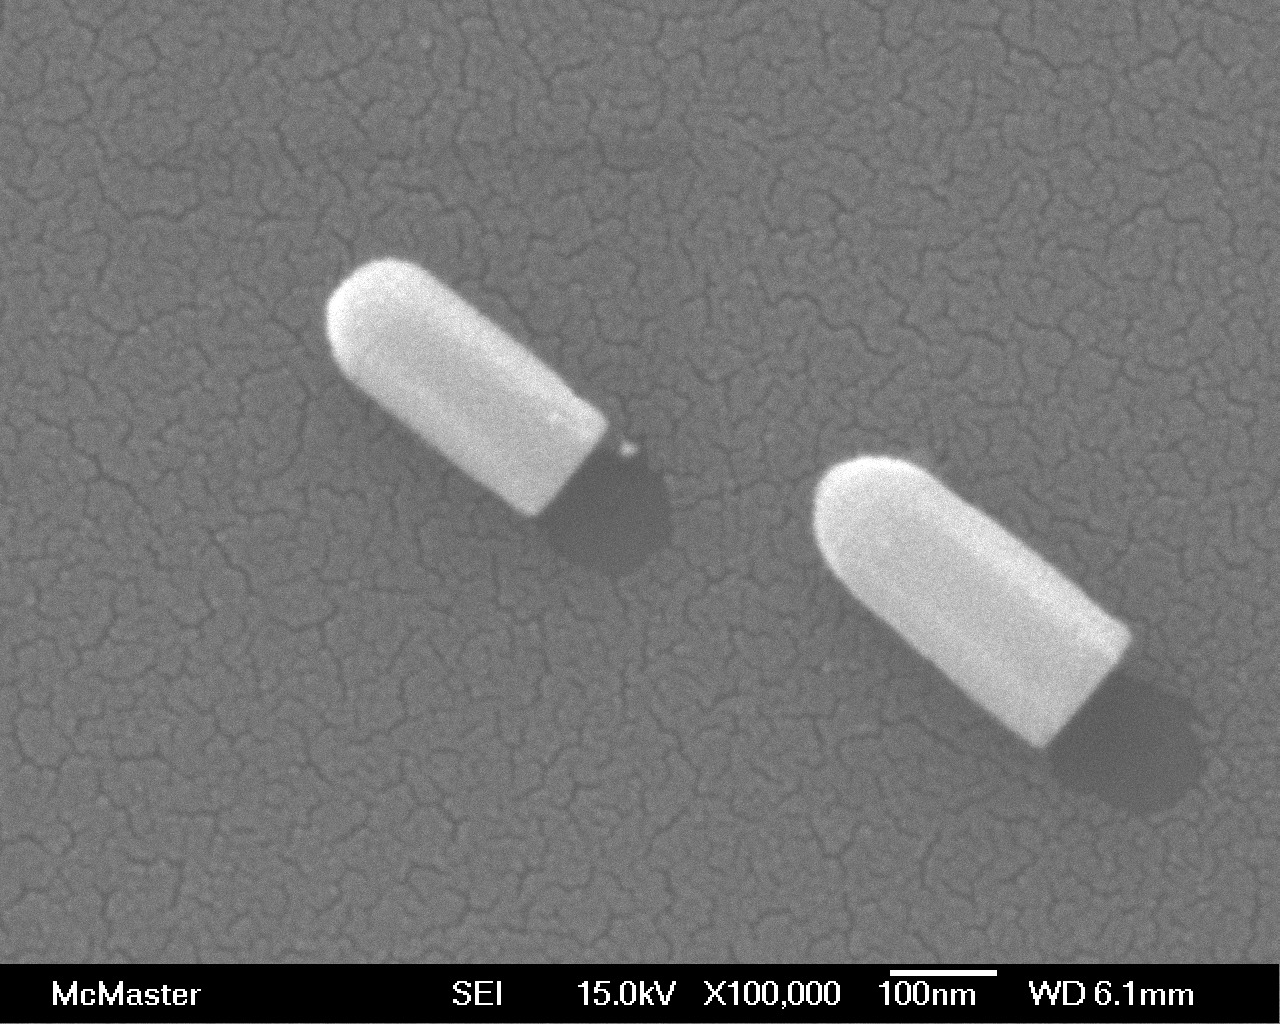
\includegraphics[width=0.8\textwidth]{cdteliftoff_nanowires}
    \caption{\label{fig:cdteliftoff_nanowires}Toppled CdTe Nanowire}
\end{figure}
This weak bonding phenomenon had been previously hinted at when CdTe nanowires were 
observed in SEM to have toppled in place, as shown in \cref{fig:cdteliftoff_nanowires}, a 
event that could not have happened unless the bond strength with the interface was very 
weak.

After the discovery of the liftoff phenomenon with lithographic patterning, simpler 
methods of liftoff were attempted. Strong adhesive tapes were found to successfully 
remove thin films with a simple mechanical peeling motion. While the tape peeling was 
effective, the large curvatures cause cleaving and breakage in the lifted off film. 
Adhesive epoxies were attempted and found to provide a more rigid carrier, eliminating 
cleaving and breakage. Yields of liftoff are highly dependent on the quality of bonding 
to the CdTe surface, clean surfaces and effective adhesives are key. Numerous other 
bonding methods were tested including optical element adhesive, polymer films and the 
simplification of liftoff by the addition of LN\textsubscript{2} as thermal shock. The generalized adhesive based liftoff process is shown in \cref{fig:cdteliftoff_process}
\begin{figure}
    \centering
    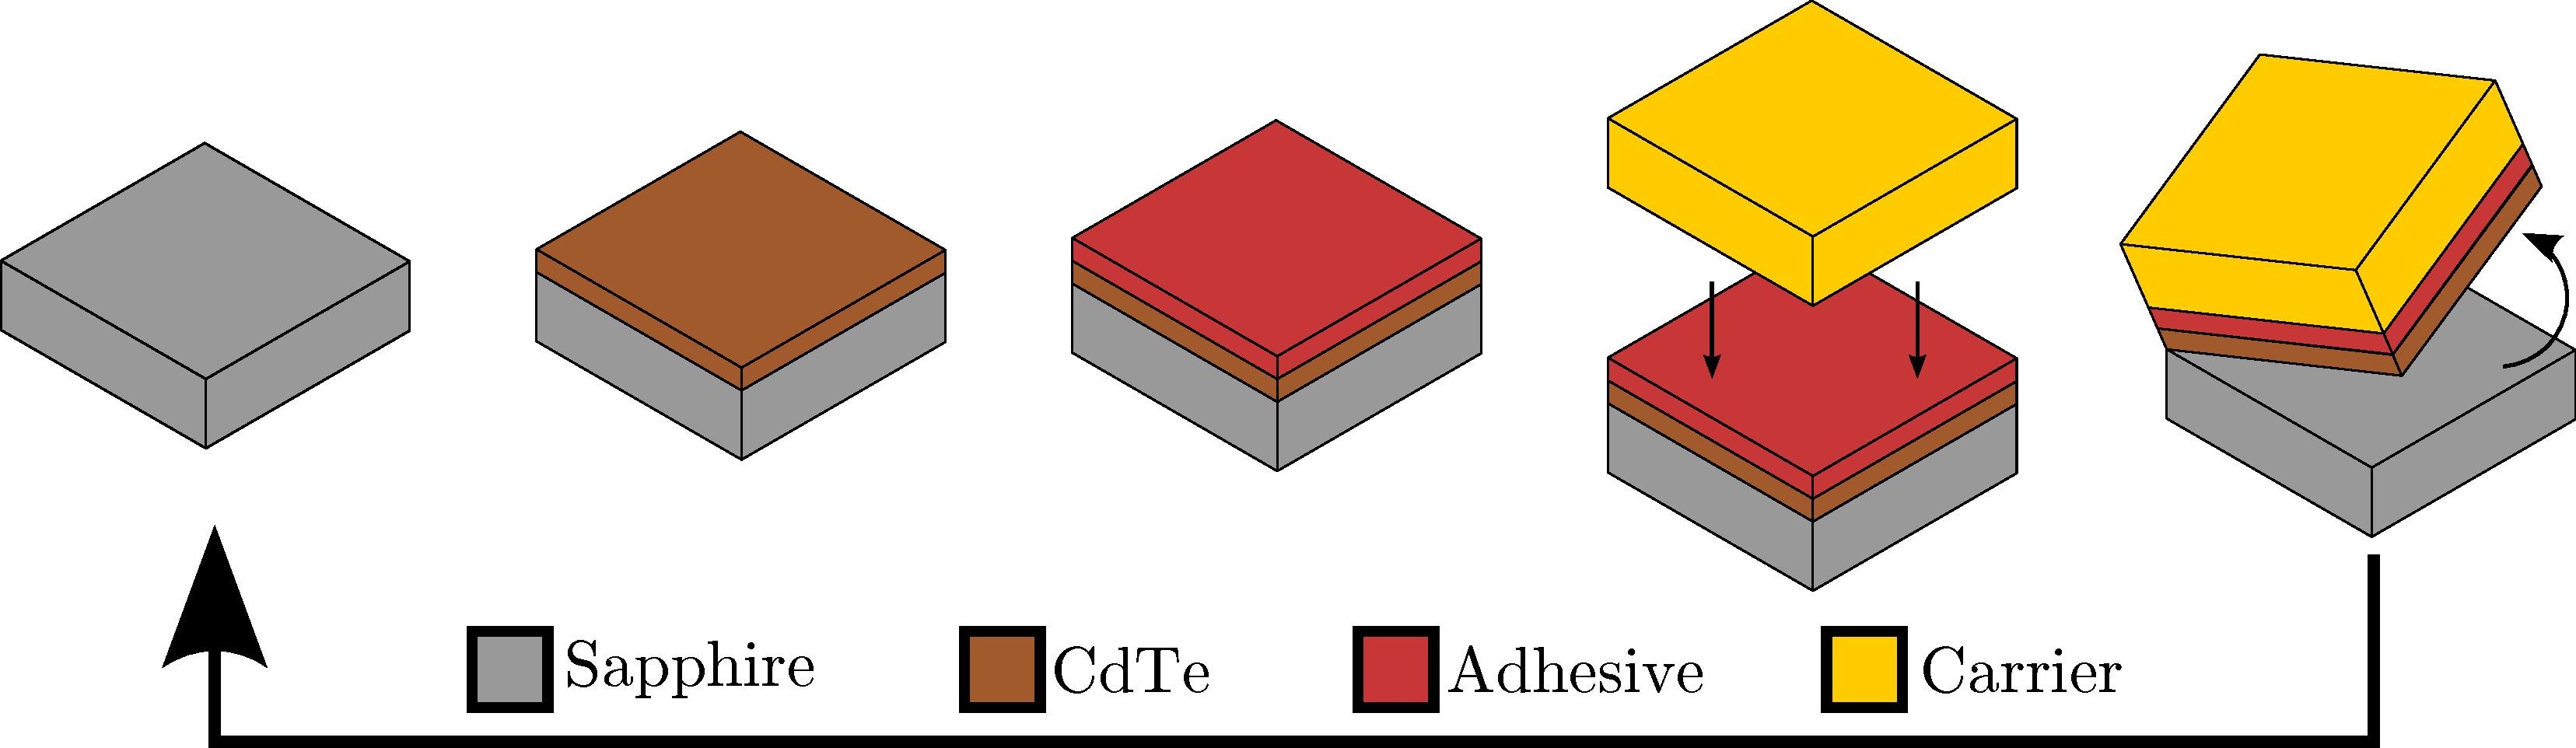
\includegraphics[width=\textwidth]{cdteliftoff_process}
    \caption{\label{fig:cdteliftoff_process}Generalized CdTe liftoff process}
\end{figure}
The flexible non-conductive liftoff carriers offered a first step to producing 
freestanding thin films, but electrical contact to the films is a key property in order 
to yield devices. To this end, thin films were coated with metal, first platinum (a known 
CdTe contact material) and then copper, in order to create a temperature stable surface. 
Samples were then wetted with solder paste and placed metal side down onto a copper 
surface, and thermally cycled through a solder reflow curve, as shown in 
\cref{fig:cdteliftoff_process}b. Upon removal from the oven, the films were found to have bonded to the copper surface and spontaneously lifted off from the original sapphire substrate. These experiments have demonstrated that the production of freestanding thin films by the liftoff phenomenon is remarkably simple and straightforward.

Concurrent to investigations into the production of freestanding thin films via the liftoff process, the obvious question arose as to the properties of these films when compared to those attached to the epitaxial substrate. 2DXRD measurements were undertaken on thin films before, \cref{fig:cdteliftoff_F22_attached} and after \cref{fig:cdteliftoff_F22_released}, liftoff processing using two part epoxy.
\begin{figure}
    \centering
    \begin{subfigure}[b]{0.45\textwidth}
        \centering
        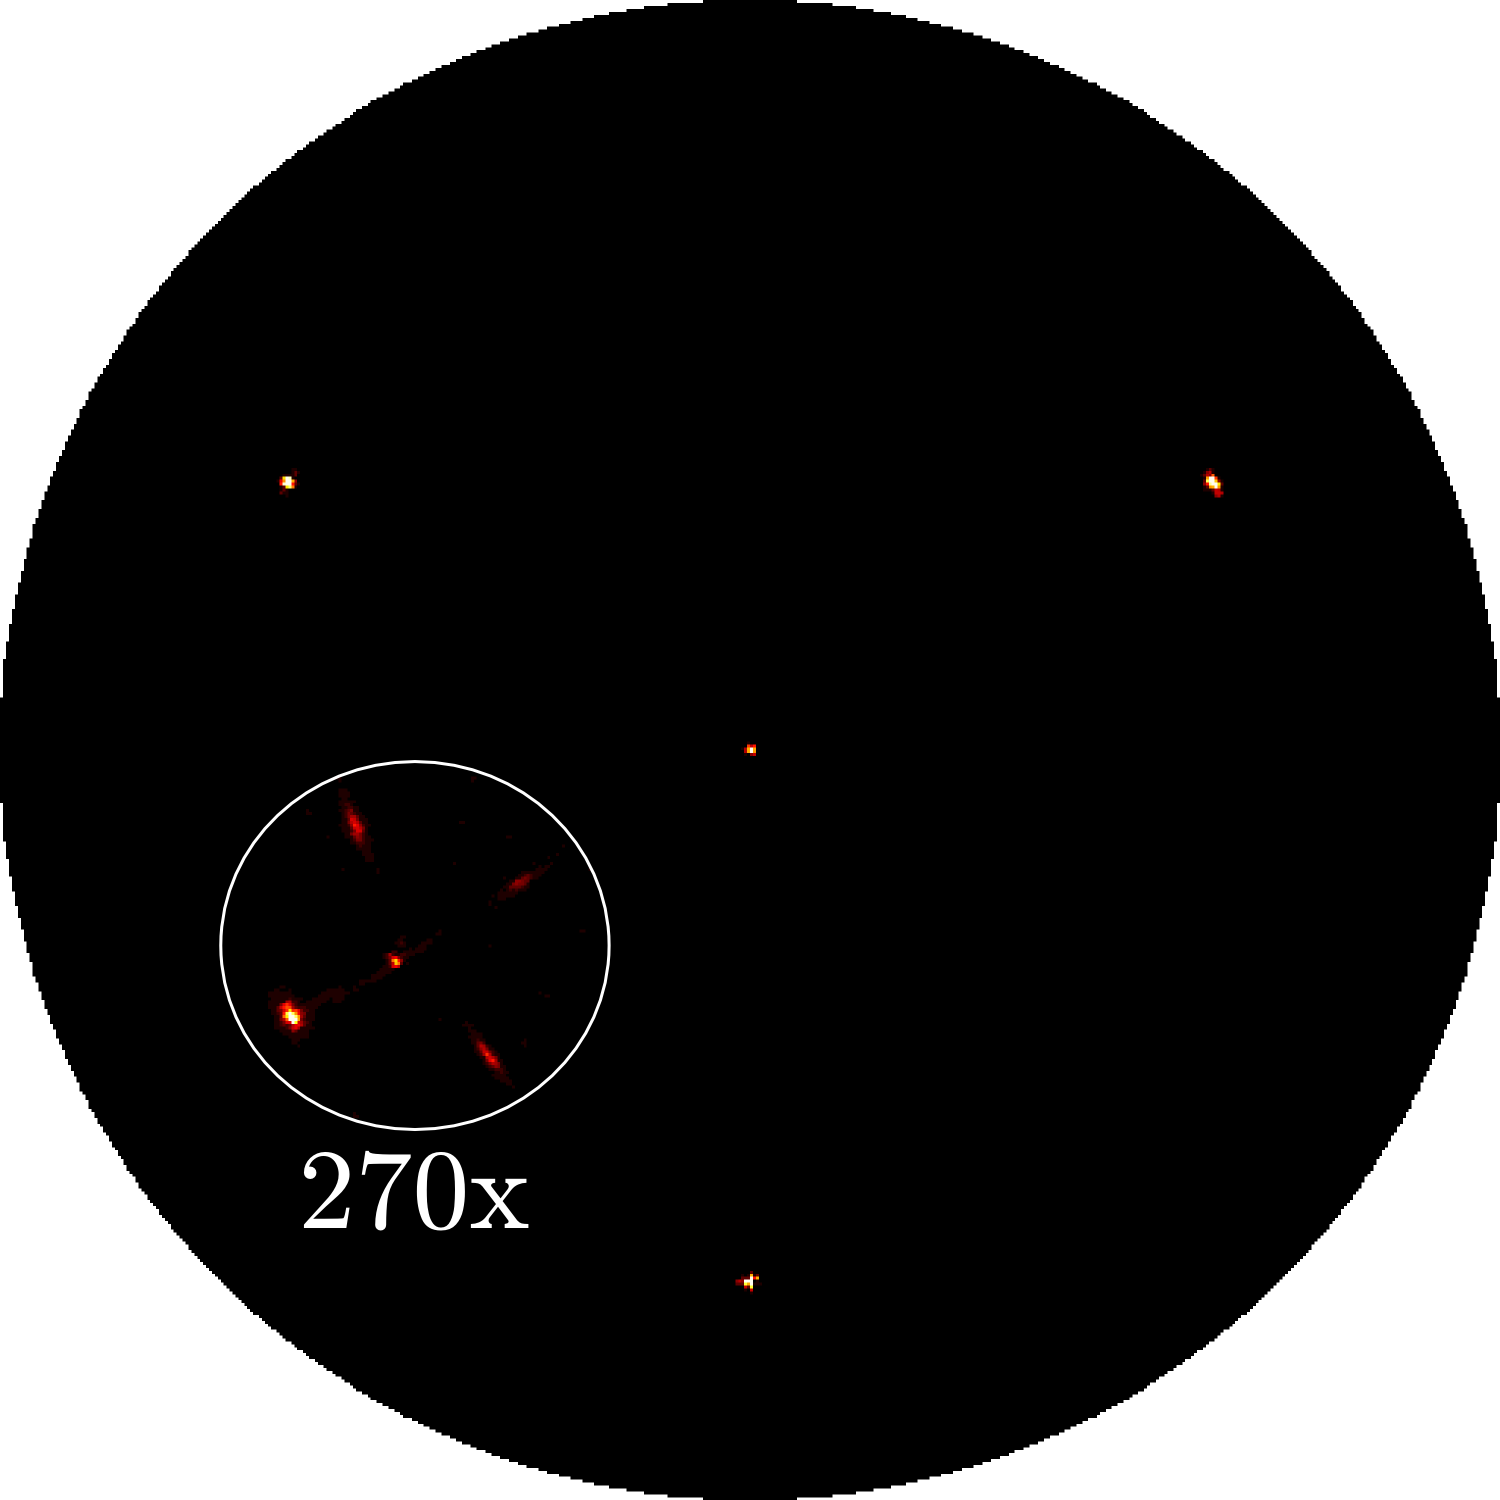
\includegraphics[width=\textwidth]{cdteliftoff_F22_attached}
        \caption{\label{fig:cdteliftoff_F22_attached}(111) Pole figure of as-grown CdTe on sapphire}
    \end{subfigure}%
    \begin{subfigure}[b]{0.45\textwidth}
        \centering
        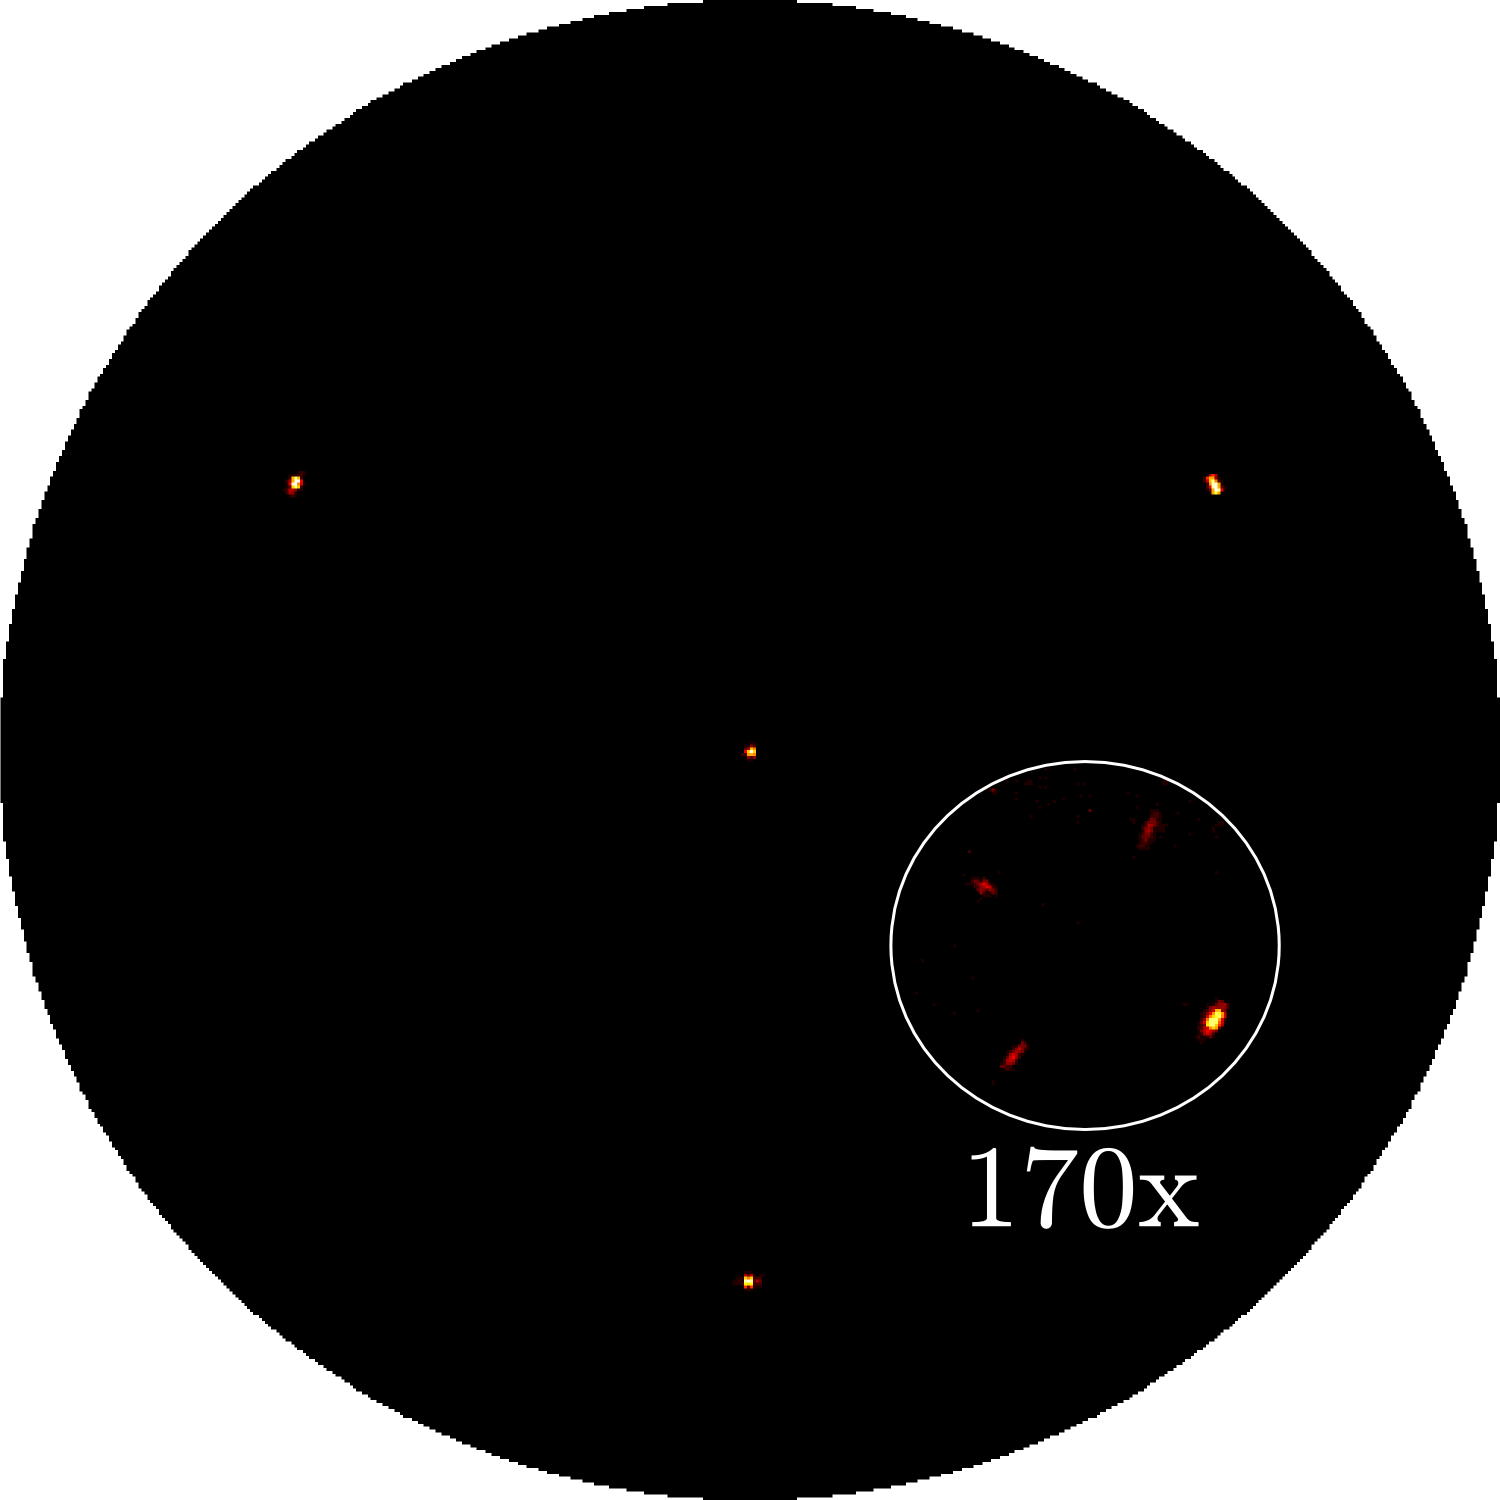
\includegraphics[width=\textwidth]{cdteliftoff_F22_released}
        \caption{\label{fig:cdteliftoff_F22_released}2DXRD of single crystal CdTe thin film on epoxy carrier}
    \end{subfigure}%
    \caption{\label{fig:cdteliftoff_2DXRD}Attached and released CdTe pole figures}
\end{figure}
2DXRD measurements of lifted off films, when compared to as-grown films, show a qualitatively identical pole figure. Peak broadness is unchanged, only the bleed through of the sapphire (024) peak disappears after the removal of the sapphire substrate. The change in the magnitude of the secondary phase is due to the change in location of the two 2DXRD measurements.

The mechanism by which liftoff of CdTe on sapphire substrates occurs has not been definitively determined. A number of theoretical models have been examined by this group to explain the exceptional interface which yields epitaxial single crystal thin film growth and then releases the resulting film with relatively little effort. The models proposed to explain such a process are 1) finite thickness polarization induced interface reorganization (a.k.a.the polarization catastrophe) 2) double layer Te nucleation, 3) van-der-waals induced epitaxy and 4) generalized weak covalent bonding.

Polar oxides (such as sapphire) are known to build up an unstable polarization due to unbalanced charge distribution (dipoles) in their unit cells, resulting in a small by finite voltage. This unstable polarization must be resolved as it builds to millions of volts over a crystal. This unstable polarization can be resolved by reorganization of the surfaces to counteract the dipole, or via charge transfer from an overlayer. Either of these mechanisms could have a significant impact on the interface between the CdTe and the sapphire. Both atomic reorganization and charge transfer have the possibility of drastically altering the bonding environment leading to the liftoff phenomenon.

Investigations by this group into the liftoff phenomenon have included the use of density functional theory (DFT) modelling of the energy landscape of Cd and Te atoms on a sapphire surface, and their preferred position. Modelling of this system has indicated a preference for two layers of Te to bond to the sapphire substrate before the atoms form the typical CdTe structure. This two-layer structure immediately at the interface may be beneficial during nucleation however after some critical thickness the CdTe grown above may influence this layer such that the bonding is significantly weakened.

Finally, it is possible that the bonding energies between the initial thin film nucleation layer and substrate to be very small, with bonding being more akin to van der waals forces than to the typical covalent or semi-ionic bonding seen in solids. The bonding is sufficiently strong enough to provide a good template for epitaxial growth, but when strong perturbative forces (thermal strains, mechanical peeling) are applied, the bonding can be overwhelmed. This weak bonding regime may be due to the strongly ionic nature of the CdTe semiconductor ($\sim$70\% ionicity) combined with the highly stable oxide surface of sapphire.
\section{Implications for Symmetry and Energy at Epitaxial Surfaces}
The interface that lies between CdTe and sapphire has been a place of great interest for the Preston research group for many years. While sapphire can be described simply using its lattice constants and space group, such a description leaves out many complicating factors.

From a symmetry point of view, the body diagonal of CdTe fits onto sapphire with two geometric orientations. This coincident surface net, where the two crystals meet, offers the initial template for alignment of the CdTe, promoting a two-phase nucleation and growth. Such orientational relationships are key for epitaxy to occur, with fewer geometric possibilities being preferred, as to reduce grain boundaries.

If growth occurred as in graphoepitaxy, where only geometry defines crystal orientation, this would still lead to defective material. From an energy point of view, the surface of sapphire can offer an energy landscape which selectively promotes one geometric orientation. For such preferences to exist, the surface must be stable and uniform, a difficult goal with the multi-layered structure of c-plane sapphire. When a uniform surface does exist, the added energy landscape is superimposed on the geometry, resulting in a single orientation being preferred for nucleation at the surface. The role of the surface energy landscape is a key factor in understanding epitaxy on more complicated surfaces such as complex oxides, as this work demonstrates that surface termination can have a strong effect on nucleation.